\documentclass[aspectratio=169]{beamer}
\usepackage{basileabeam}

% Notes:
%\pgfpagesuselayout{2 on 1}[a4paper,border shrink=5mm]
%\setbeamertemplate{note page}[plain]
%\setbeameroption{show notes on second screen=bottom}

\title              {Cuteserver}

\author             {Rahel Kempf, Ephraim Siegfried}
\institute          {Operating Systems, University of Basel}

\date               {14.6.2024}

\ulogo        		{Template/header}
\ulistelement    	{Template/listelement}

\graphicspath{{Figures/}}

% Options:
\totalNoSlidesDisabled % To turn off the total number of slides in the footer. Comment this if you want the total number of slides in the footer

\headerSectionsDisabled % Comment this if you want a fancy header containing your sections.


\begin{document}

\begin{frame}[t,plain]
\titlepage
\end{frame}

\note{Notes can help you to remember important information. Turn on the notes option.}

\section{Section 1}	% You can also have slides prior to the first section or work entirely without sections.

\begin{frame}[c]{Progress Pictues}
  \centering
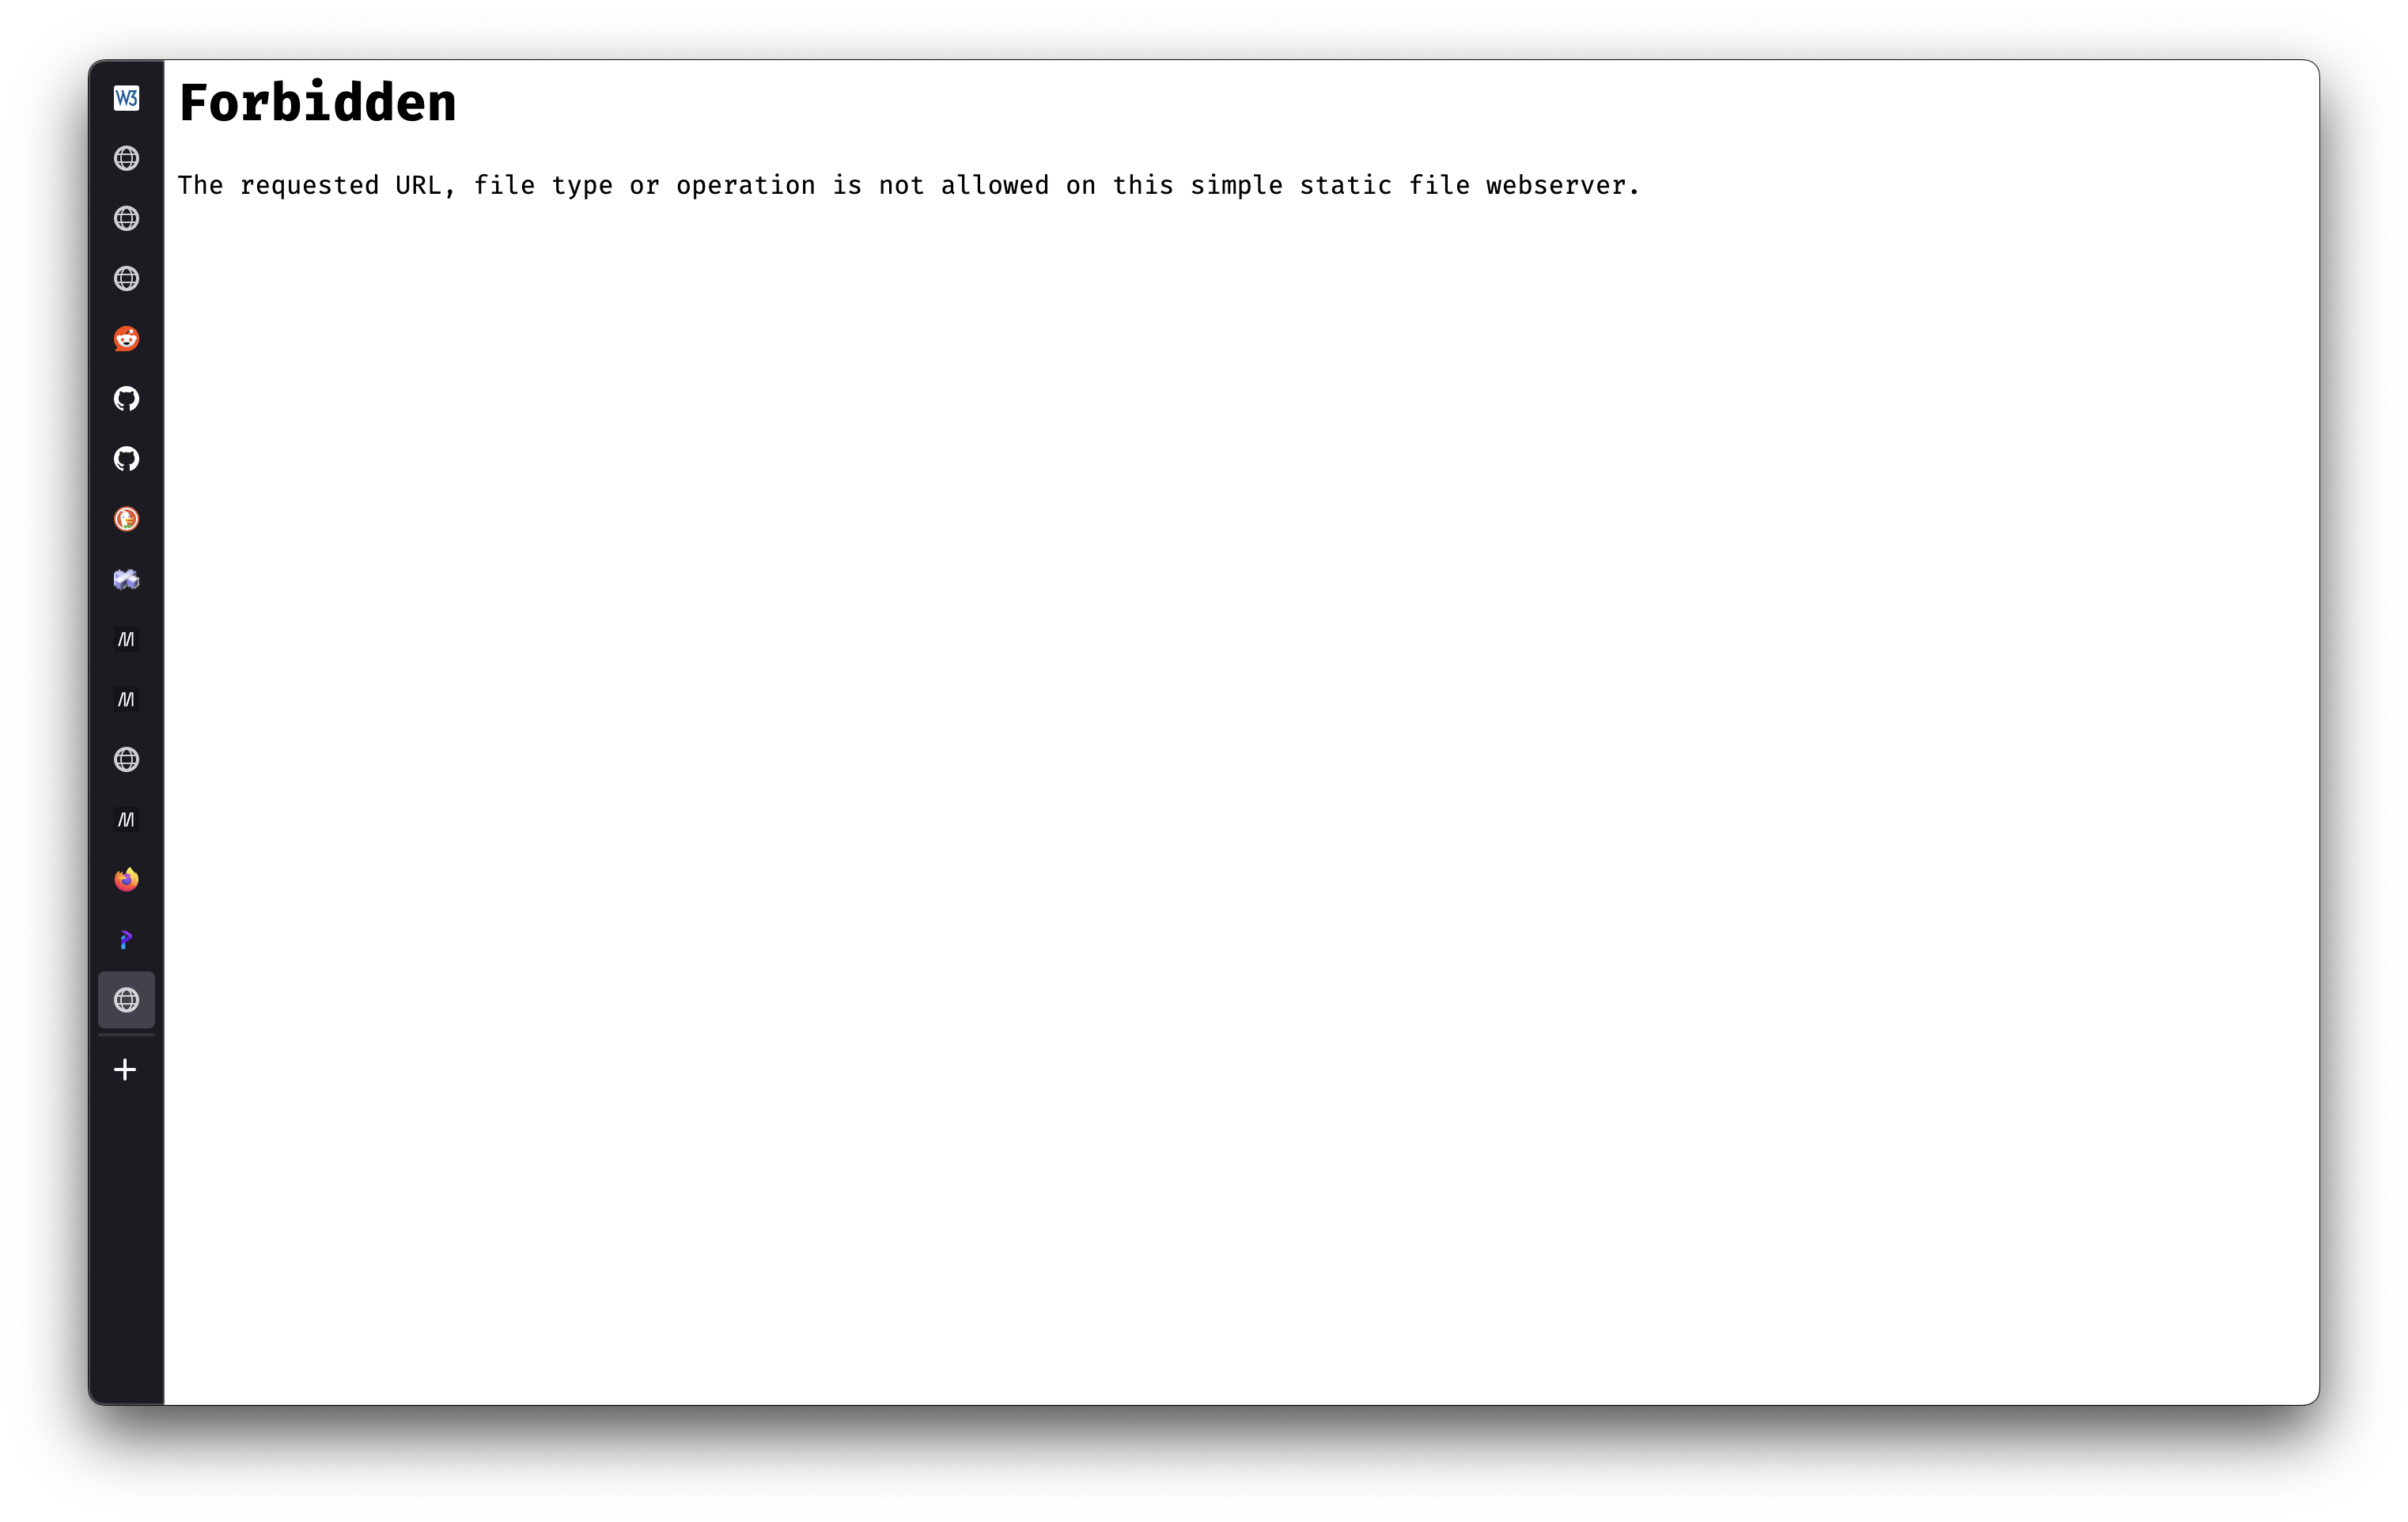
\includegraphics[width=0.8\textwidth]{00_errors.png}
\end{frame}

\begin{frame}[c]{}
  \centering

\includegraphics[width=0.8\textwidth]{00_errors1.png}
\end{frame}

\begin{frame}[c]{}
  \centering
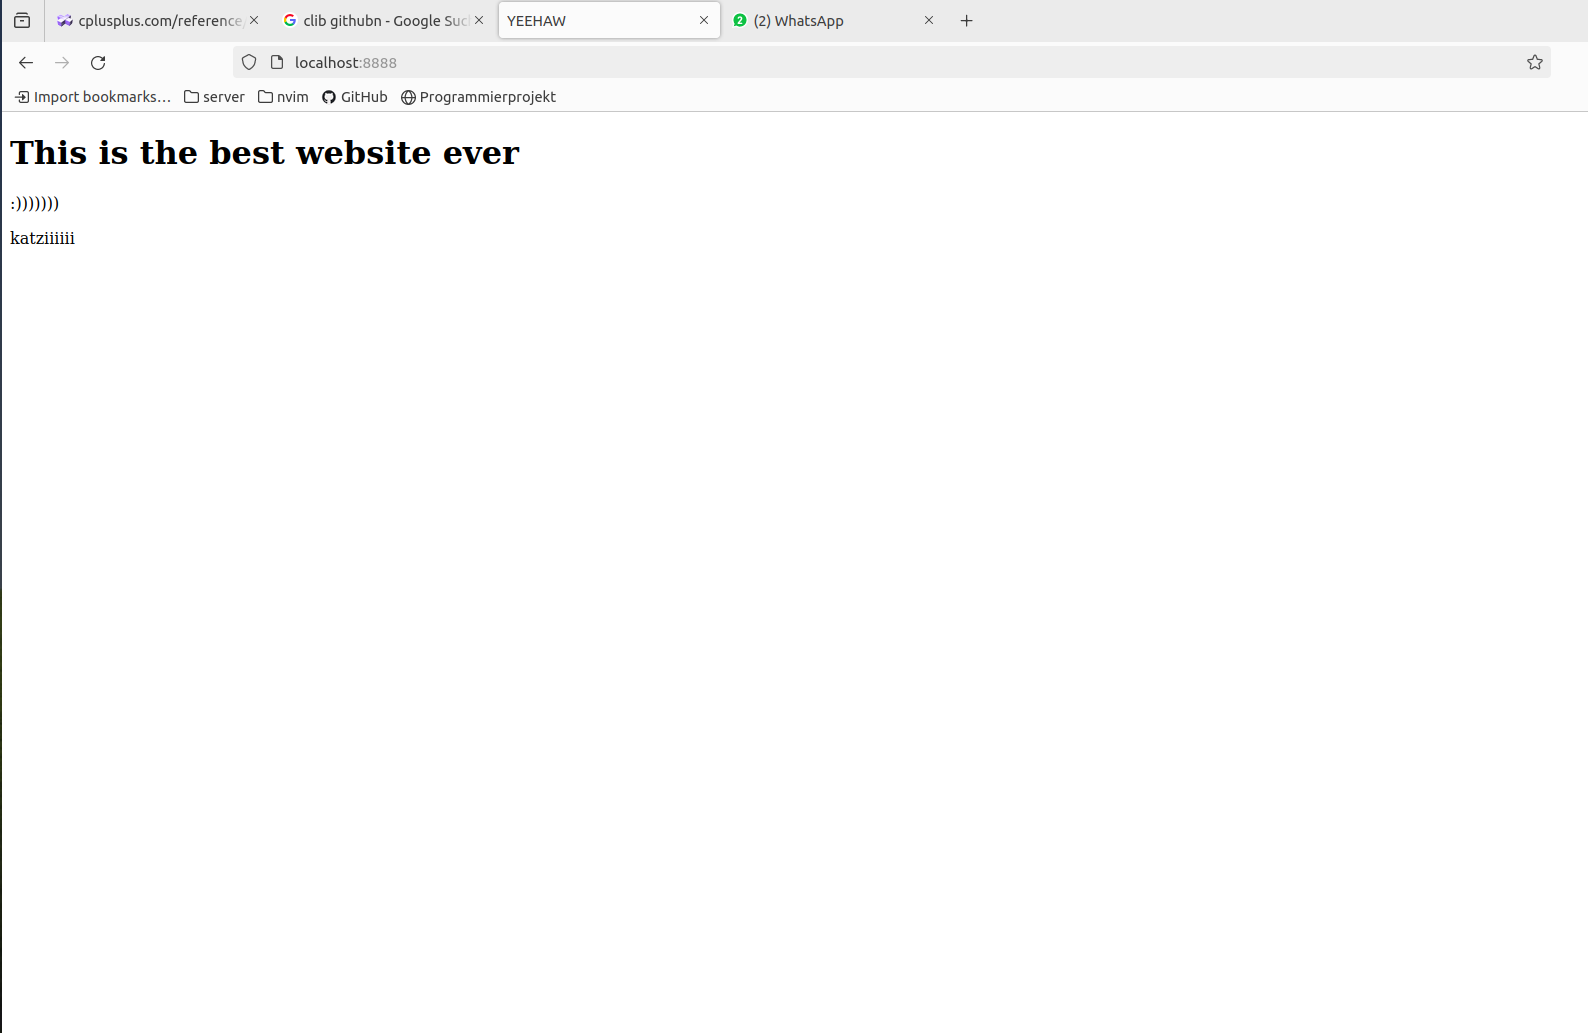
\includegraphics[width=0.8\textwidth]{01_bare_html.png}
\end{frame}

\begin{frame}[c]{}
  \centering
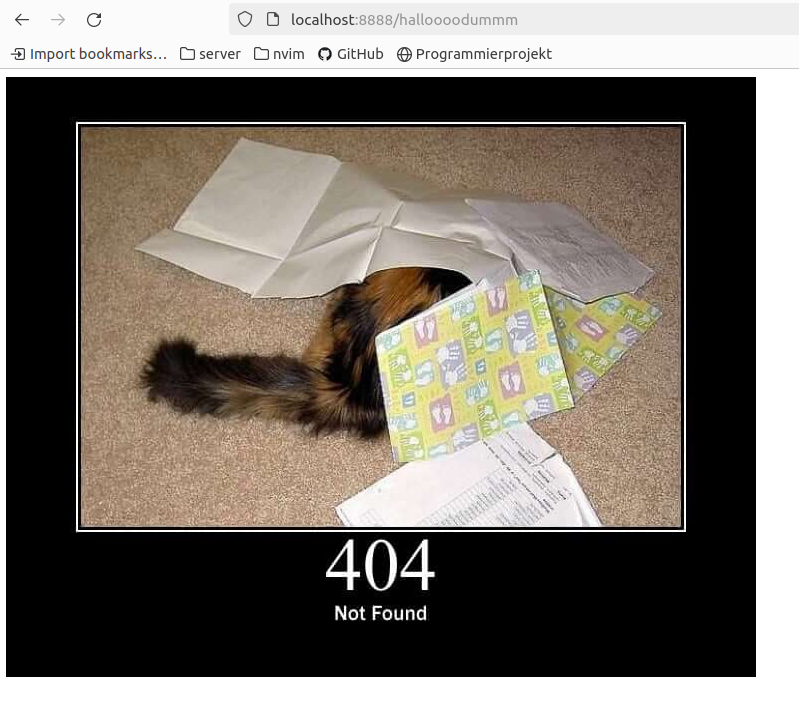
\includegraphics[width=0.8\textwidth]{02_http_cats.png}
\end{frame}

\begin{frame}[c]{}
  \centering
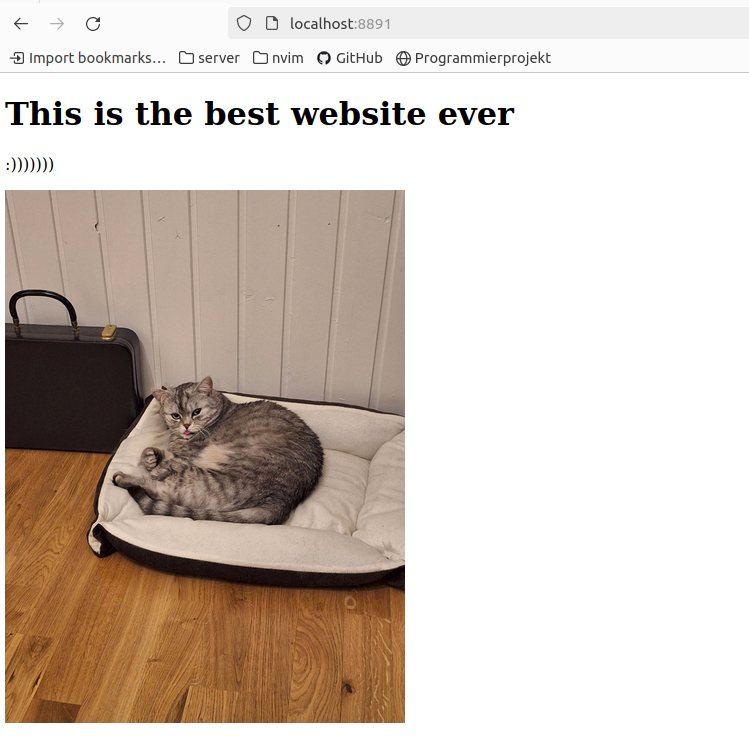
\includegraphics[width=0.8\textwidth]{03_html_mit_bild.png}
\end{frame}

\begin{frame}[c]{}
  \centering
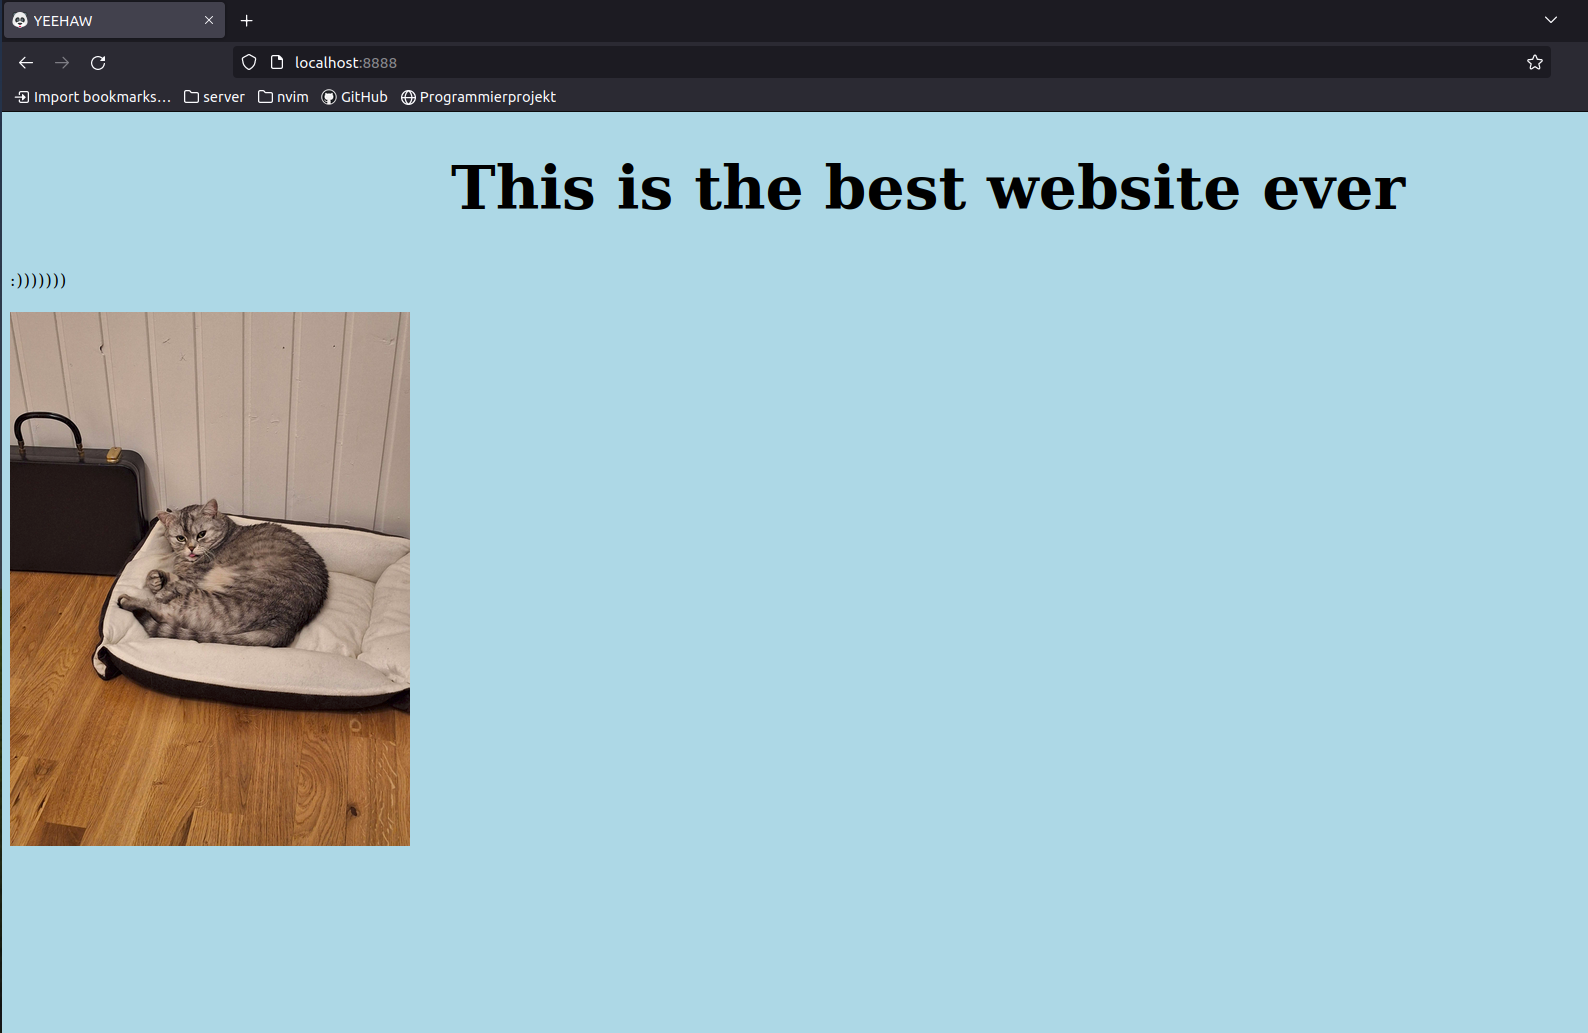
\includegraphics[width=0.8\textwidth]{04_somecss.png}
\end{frame}

\begin{frame}[c]{}
  \centering

\includegraphics[width=0.8\textwidth]{05_firstCGI.png} %TODO: ADD CGI PICTURE WITH ENV VARS
\end{frame}

\begin{frame}[c]{}
  \centering
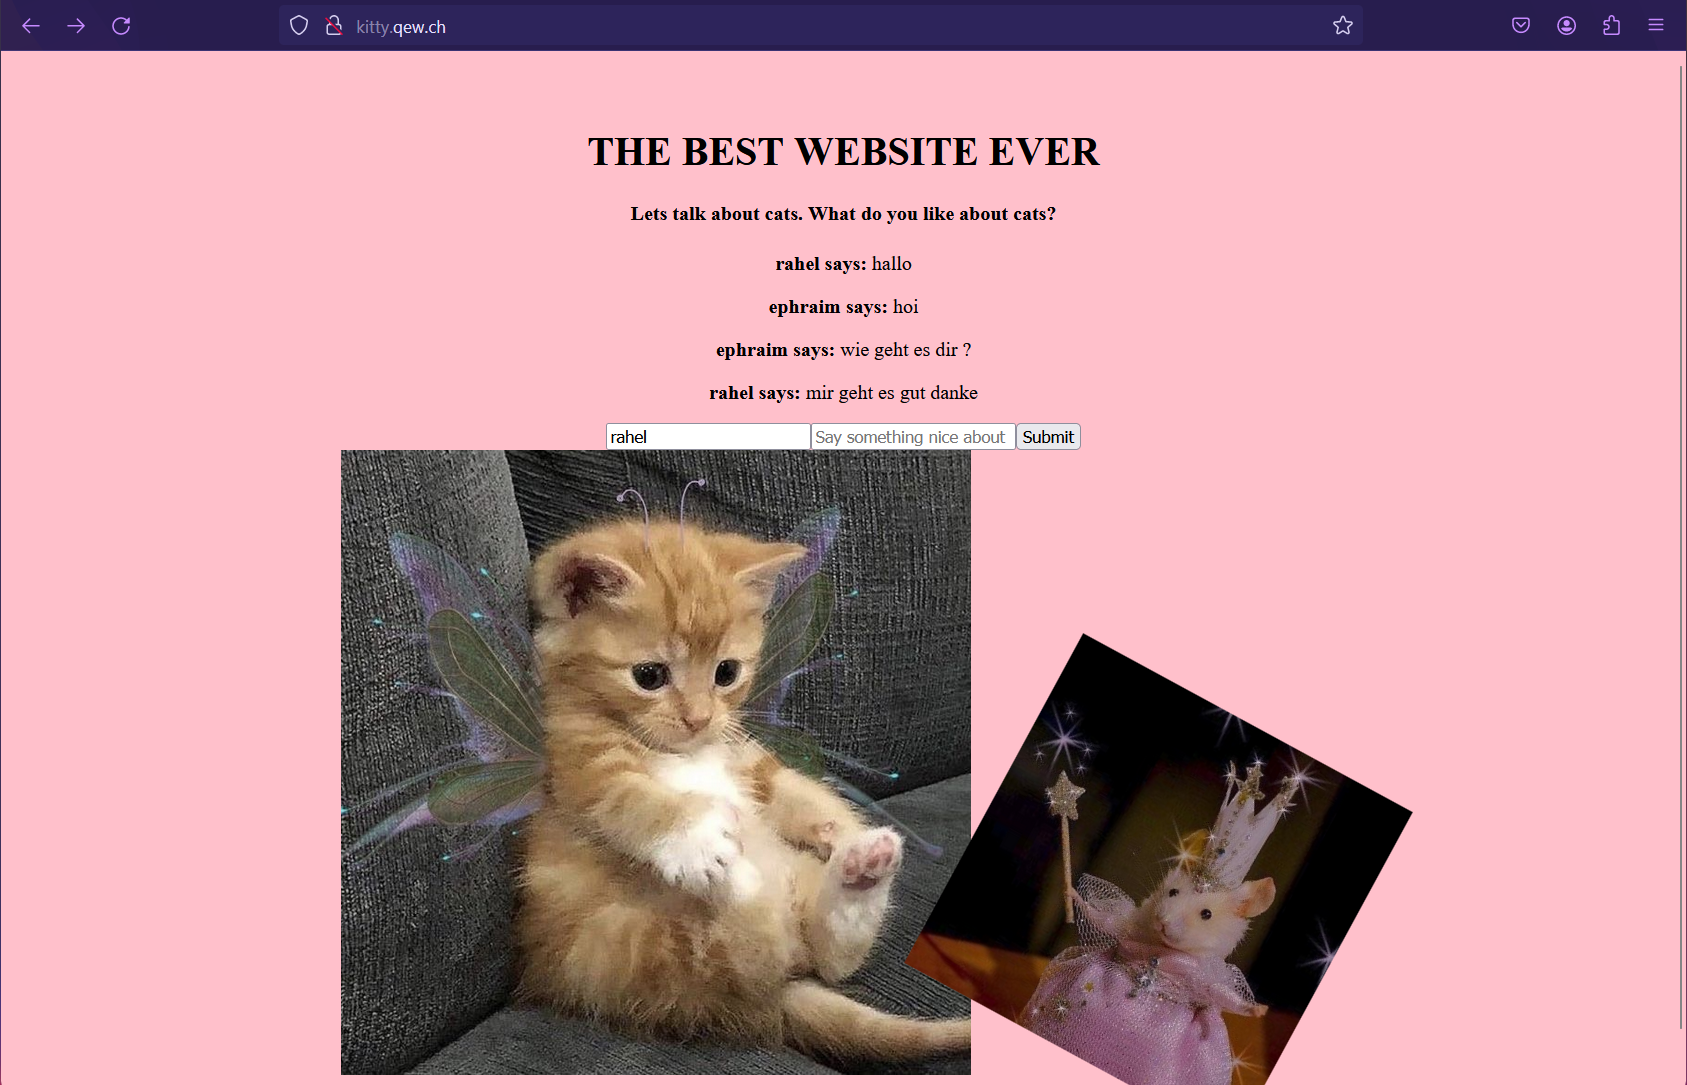
\includegraphics[width=0.8\textwidth]{06_ephi_app.png}
\end{frame}

\begin{frame}[c]{}
  \centering
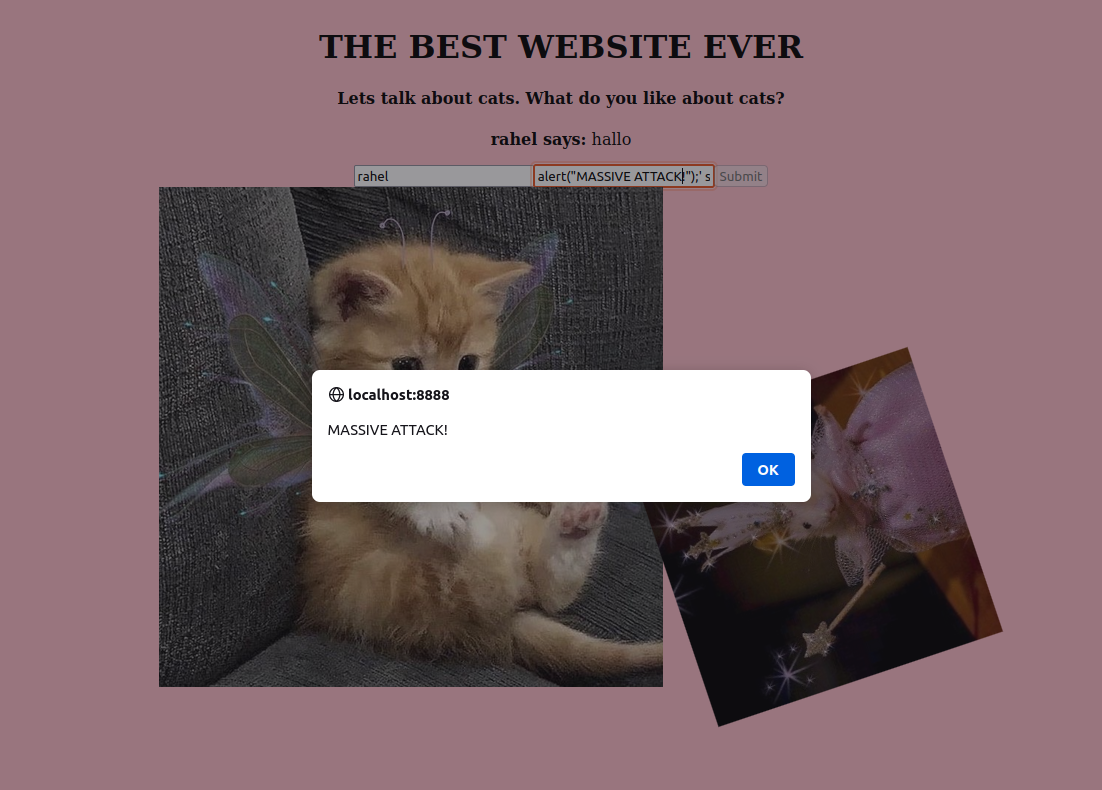
\includegraphics[width=0.8\textwidth]{07_css.png}
\end{frame}

\note{Notes can help you to remember important information. Turn on the notes option.}

\section{Section 2}

\begin{frame}[t,plain]
  \lastpage{{\usebeamerfont{title} Questions?}}
\end{frame}

\end{document}

